\begin{figure}[htbp]
\centering
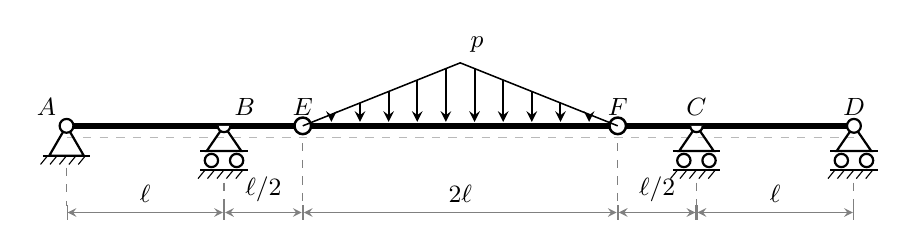
\begin{tikzpicture}[>=stealth, line width=0.8pt, font=\small,
	nodo/.style  = {circle, fill=white, draw=black,
		inner sep=0pt, minimum size=5pt, line width=0.8pt},
	cint/.style  = {circle, fill=white, draw=black,
		inner sep=0pt, minimum size=6pt, line width=0.9pt},
	richiam/.style = {thin, gray, dashed},
	]
	
	%% ── Parametri geometrici ─────────────────────────────────────────────────
	%% Unità: L = ell.  Posizioni:
	%%   A=0, B=L, E=1.5L, mez=2.5L, F=3.5L, C=4L, D=5L
	\def\L{2.00}     % ell
	\def\tw{0.22}    \def\thA{0.38}  \def\thR{0.32}
	\def\sr{0.08}    \def\bw{0.16}   \def\gw{0.30}
	\def\yd{-1.10}   % quota quotatura
	
	%% Posizioni nodi
	\pgfmathsetmacro{\xB}{\L}
	\pgfmathsetmacro{\xE}{1.5*\L}
	\pgfmathsetmacro{\xMez}{2.5*\L}   % mezzeria EF
	\pgfmathsetmacro{\xF}{3.5*\L}
	\pgfmathsetmacro{\xC}{4*\L}
	\pgfmathsetmacro{\xD}{5*\L}
	
	%% ── Trave ────────────────────────────────────────────────────────────────
	\draw[line width=2.2pt](0,0)--(\xD,0);
	
	%% ── Fibre inferiori ──────────────────────────────────────────────────────
	\draw[line width=0.6pt, dashed, gray!55](0,-0.15)--(\xD,-0.15);
	
	%% ── Etichette nodi ───────────────────────────────────────────────────────
	\node[above left =0.04]at(0,0){$A$};
	\node[above right=0.04]at(\xB,0){$B$};
	\node[above=0.12]at(\xE,0){$E$};
	\node[above=0.12]at(\xF,0){$F$};
	\node[above=0.04]at(\xC,0){$C$};
	\node[above=0.04]at(\xD,0){$D$};
	
	%% ── Cerniera A ───────────────────────────────────────────────────────────
	\draw(0,0)--++(-\tw,-\thA)--++(2*\tw,0)--cycle;
	\draw(-\gw,-\thA)--(\gw,-\thA);
	\foreach \x in {-0.24,-0.12,0,0.12,0.24}
	\draw[thin](\x,-\thA)--++(-.09,-.11);
	\node[nodo]at(0,0){};
	
	%% ── Appoggio intermedio B ────────────────────────────────────────────────
	\draw(\xB,0)--++(-\tw,-\thR)--++(2*\tw,0)--cycle;
	\draw(\xB-\gw,-\thR)--(\xB+\gw,-\thR);
	\draw(\xB-\bw,-\thR-0.12)circle(2.4pt);
	\draw(\xB+\bw,-\thR-0.12)circle(2.4pt);
	\draw(\xB-\gw,-\thR-0.24)--(\xB+\gw,-\thR-0.24);
	\foreach \x in {-0.24,-0.12,0,0.12,0.24}
	\draw[thin](\xB+\x,-\thR-0.24)--++(-.09,-.11);
	\fill[white](\xB-\sr,0)arc(180:360:\sr)--cycle;
	\draw(\xB-\sr,0)arc(180:360:\sr);
	
	%% ── Appoggio intermedio C ────────────────────────────────────────────────
	\draw(\xC,0)--++(-\tw,-\thR)--++(2*\tw,0)--cycle;
	\draw(\xC-\gw,-\thR)--(\xC+\gw,-\thR);
	\draw(\xC-\bw,-\thR-0.12)circle(2.4pt);
	\draw(\xC+\bw,-\thR-0.12)circle(2.4pt);
	\draw(\xC-\gw,-\thR-0.24)--(\xC+\gw,-\thR-0.24);
	\foreach \x in {-0.24,-0.12,0,0.12,0.24}
	\draw[thin](\xC+\x,-\thR-0.24)--++(-.09,-.11);
	\fill[white](\xC-\sr,0)arc(180:360:\sr)--cycle;
	\draw(\xC-\sr,0)arc(180:360:\sr);
	
	%% ── Carrello D ───────────────────────────────────────────────────────────
	\draw(\xD,0)--++(-\tw,-\thR)--++(2*\tw,0)--cycle;
	\draw(\xD-\gw,-\thR)--(\xD+\gw,-\thR);
	\draw(\xD-\bw,-\thR-0.12)circle(2.4pt);
	\draw(\xD+\bw,-\thR-0.12)circle(2.4pt);
	\draw(\xD-\gw,-\thR-0.24)--(\xD+\gw,-\thR-0.24);
	\foreach \x in {-0.24,-0.12,0,0.12,0.24}
	\draw[thin](\xD+\x,-\thR-0.24)--++(-.09,-.11);
	\node[nodo]at(\xD,0){};
	
	%% ── Cerniere interne E e F ───────────────────────────────────────────────
	\node[cint]at(\xE,0){};
	\node[cint]at(\xF,0){};
	
	%% ── Carico triangolare su EF ─────────────────────────────────────────────
	%% p(z) = (p/ell)*z  per 0<=z<=ell,  p(z)= p*(2-z/ell) per ell<=z<=2*ell
	%% ell = L,  altezza massima = hP
	\def\hP{0.80}   % altezza grafica picco p (cm)
	\def\nArr{11}   % numero di frecce
	
	%% contorno del diagramma di carico (linea superiore)
	\draw[line width=0.55pt,black]
	(\xE,0)
	-- (\xMez,\hP)
	-- (\xF,0);
	
	%% frecce verticali distribuite
	\foreach \k in {0,1,...,\nArr}{
		\pgfmathsetmacro{\t}{\k/\nArr}           % t in [0,1], x in [xE, xF]
		\pgfmathsetmacro{\xx}{\xE + \t*2*\L}      % x globale
		% intensità: tenda con picco in t=0.5
		\pgfmathsetmacro{\hh}{\hP*(1 - abs(2*\t - 1))}
		\ifdim\hh pt > 0.06pt
		\draw[->,>=stealth,line width=0.7pt](\xx,\hh)--(\xx,0.05);
		\fi}
	
	%% etichetta p
	\node[font=\small,above right=0.02]at(\xMez,\hP){$p$};
	
	%% ── Quotatura ─────────────────────────────────────────────────────────────
	\draw[richiam](0,-\thA-0.15)--(0,\yd+0.08);
	\draw[richiam](\xB,-\thR-0.40)--(\xB,\yd+0.08);
	\draw[richiam](\xE,-0.22)--(\xE,\yd+0.08);
	\draw[richiam](\xF,-0.22)--(\xF,\yd+0.08);
	\draw[richiam](\xC,-\thR-0.40)--(\xC,\yd+0.08);
	\draw[richiam](\xD,-\thR-0.40)--(\xD,\yd+0.08);
	
	\draw[thin,gray,|<->|](0,\yd)--(\xB,\yd);
	\node[font=\small,above=0.04]at(0.5*\xB,\yd){$\ell$};
	
	\draw[thin,gray,|<->|](\xB,\yd)--(\xE,\yd);
	\node[font=\small,above]at(0.5*\xB+0.5*\xE,\yd){$\ell/2$};
	
	\draw[thin,gray,|<->|](\xE,\yd)--(\xF,\yd);
	\node[font=\small,above]at(0.5*\xE+0.5*\xF,\yd){$2\ell$};
	
	\draw[thin,gray,|<->|](\xF,\yd)--(\xC,\yd);
	\node[font=\small,above]at(0.5*\xF+0.5*\xC,\yd){$\ell/2$};
	
	\draw[thin,gray,|<->|](\xC,\yd)--(\xD,\yd);
	\node[font=\small,above]at(0.5*\xC+0.5*\xD,\yd){$\ell$};
	
\end{tikzpicture}
\caption{Trave di Gerber su quattro appoggi ($n_a=4$, $n_e=5$,
	$n_c=2$): cerniera in $A$, appoggi continui in $B$ e $C$,
	carrello in $D$, cerniere interne in $E$ e $F$.
	Luci: $AB = CD = \ell$, $BE = FC = \ell/2$, $EF = 2\ell$.
	La campata portata $EF$ è soggetta a un carico trasversale
	triangolare di intensità massima $p$ nella sezione di mezzeria
	e nulla agli estremi $E$ e $F$.}
\label{fig:gerber_esempio_schema}
\end{figure}
